%	LaTeX template for the Collaborative Research Center proposal (3rd funding period) Oxyflame.
%	WSA, RWTH Aachen, 2020, (contact person: Stefan Pielsticker)

%%%% PLEASE ADJUST:
%\WorkInstruction{ Enter the number of the project here. Replace only the text "Example project" Please make sure that the project name corresponds exactly to the name of the folder of your project.}
% Example: \renewcommand{\Project}{A1}

\renewcommand{\Project}{A1}
\renewcommand{\ChapterTitle}{Gasphase modelling}
\renewcommand{\ProjectTitle}{Original title from DFG proposal}

\newcommand*\positioncircle[1]{\raisebox{.5pt}{\textcircled{\raisebox{-.9pt} {#1}}}}


%%%% DON'T CHANGE ANYTHING FROM HERE UNTIL NEXT MARKER!
\chapter{\ChapterTitle}
%%%% DONT CHANGE ANYTHING UNTIL HERE!

%%%% PLEASE ADJUST:
\chapterauthor[1]{Anita Meraviglia}
\chapterauthor[1]{Pooria Farmand}
\chapterauthor[2]{Leon Loni Berkel}
\chapterauthor[3]{Stefan Pielsticker}
\chapterauthor[3]{Reinhold Kneer}
\chapterauthor[2]{Christian Hasse}
\chapterauthor[1]{Heinz Pitsch}

%%%% DON'T CHANGE ANYTHING FROM HERE UNTIL NEXT MARKER!
\begin{affils}
	%%%% DONT CHANGE ANYTHING UNTIL HERE!
	
	%%%% PLEASE ADJUST:
	\chapteraffil[1]{\RWTHITV}
	\chapteraffil[2]{\RWTHWSA}
	
%%%% DON'T CHANGE ANYTHING FROM HERE UNTIL NEXT MARKER!
\end{affils}
\begin{refsection}

\begin{abstract}
\label{sec:\Project _Abstract}
%%%% DONT CHANGE ANYTHING UNTIL HERE!

%%%% PLEASE ADJUST
%\WorkInstruction{Title: Keep it short and make sure that it fits well with the part title and the other project titles within that part. Therefore see the planned chapter outline in section~\ref{ex: chap Outline}.}

%\WorkInstruction{Author List: If you use data from FP1/FP2 members, please list them here as well.}

%\WorkInstruction{Affiliations: Please use the commands already prepared (\textbackslash RWTHWSA, \textbackslash RWTHAIA, \textbackslash RWTHITV, \textbackslash RUBLEAT, \textbackslash RUBLTC, \textbackslash RUBThermo, \textbackslash RUBTC, \textbackslash RUBACII, \textbackslash TUDSTFS,\textbackslash TUDRSM, \textbackslash TUDEST. For changes or other affiliations text us.}

\blindtext[2]

\WorkInstruction{Put abstract here, not longer than first page.}

\end{abstract}


\newpage % Christian
\section{Introduction} 
Chemical kinetic models are essential when dealing with combustion phenomena as they provide crucial information regarding reaction rates, species transport, and temperature effects. In chapter~\ref{\Project_B3}, solid particle DNS are performed to analyse the combustion and ignition behaviour as well as the main \ce{NO_x} formation pathways in the partially premixed flame, resulting from the combustion of a single solid particle of coal and biomass under high-temperature air and oxy-fuel conditions at atmospheric pressure. Therefore, with this application in mind, it is necessary to develop a chemical kinetic model to describe the underlying chemistry of the released volatile species in the surrounding gas phase of the solid particle. The latter is determined by employing the solid particle model for coal and biomass devolatilisations from Cha.~\ref{\Project_A8}, which leads to the definition of a complex mixture ranging from light hydrocarbons and oxygenated species up to heavy lignin tars (\ce{C24H28O4}) and aromatic compounds. Additionally, various nitrogen-containing species are present, and the introduction in the kinetic model of the relevant chemistry describing their evolution in the combustion system is essential for accounting for the primary \ce{NO_x} formation pathways.
% mehr .. Oxyflame bezogen ... not only B3 ...
% Chen2022 => B1???
\\
Detailed chemical kinetic models aim to describe the combustion process as accurately as possible. However, this might require hundreds or even thousands of species and reactions. Since the computational cost of complex simulations typically increases as the number of species in the employed kinetic model grows, developing skeletal kinetic models with a reduced number of species and reactions while preserving high accuracy is of key importance for performing the simulation of interest that would be otherwise computationally prohibitive.
\\
Why we need new models and L.Cai ... => focus on oxyconditions and combined with solid model
 

% why we need new chemcial kinetic models: Not only B3 more ...


%\textbf{Chemical kinetic model development}
%\begin{itemize}
%	\item Detailed Chemical kinetic models (ITV-2019 and ITV-2023)
%	\begin{itemize}
%		\item Development of the reduced ITV model (Cai 2020)			% ? one to the top ...
%		\item Development of recent kinetic model
%	\end{itemize}
%	\item Skeletal chemical kinetic model
%	\item Development of \ce{NOx} chemical kinetic submodel
%\end{itemize}
% 
%\textbf{Validation of the kinetic models}
%\begin{itemize}
%	\item Skeletal kinetic model for coal combustion
%	\begin{itemize}
%		\item ITV-2019 (Cai 2020)
%		\item ITV-2023
%	\end{itemize}
%	\item Skeletal kinetic model for biomass combustion
%	\item Validation of \ce{NOx} chemical kinetic submodel
%\end{itemize}
 
 
\section{Chemical kinetic model development}
The development of suitable chemical kinetic models for the gas phase kinetics with an compact model size is presented in this section. ...

%very brief here. Cai and we developed this and that ... Structured as follows ..



\subsection{Development of the reduced ITV model}
Liming Cai: paper ???
\\
Different development process ...
 % Liming Cai ????
 
 
 
\subsection{Development of recent kinetic models}
The development of recent skeletal kinetic models for coal and biomass combustion involves a multi-step reduction strategy using detailed chemical kinetic models. A schematic of the whole reduction strategy is summarized in Fig.~\ref{fig:B1bKineticModelDevelopmentStructure}.
\\
In the first step, detailed chemical kinetic models have been developed by integrating the chemistry of the missing volatile species from coal and biomass combustion into the model of Langer et al.~\cite{Langer2023}. The model from Langer et al.~\cite{Langer2012} has been systematically extrapolated from recently published chemical kinetic models and combined with recently published detailed chemical kinetic models~\cite{Wagnon2018, Debiagi2016, Pelucchi2015}, describing the missing volatile species chemistry. The so obtained kinetic models will be referred to as "Merged-ITV-Cellulose", "Merged-ITV-Propionaldehyde", and "Merged-ITV-Anisole", as shown in Fig.~\ref{fig:B1bKineticModelDevelopmentStructure}. Details about this development step will be given later. The obtained models undergo a multi-step reduction strategy involving Direct Relation Graph with Error Propagation (DRGEP)method and Reaction Flux Analysis (RFA). Skeletal kinetic models from each reduction step will be named employing the prefixes "DRGEP-Skeletal" and "RFA-Skeletal", followed by the name of the corresponding detailed chemical kinetic model. The reduction process allows the retention of only the relevant chemistry for the species of interest. This allows the merging process of the skeletal models to be more straightforward, leading to a compact chemical kinetic model (ITV-compact) able to accurately describe the evolution of the volatile species released from coal and biomass. The obtained compact model is further divided into two skeletal kinetic models via DRGEP and RFA. These skeletal kinetic models describe the gas phase kinetics of volatile species released from coal (Skeletal-ITV-Coal) and biomass (Skeletal-ITV-Bio).
\begin{figure}[h]
  \centering
  \subfloat{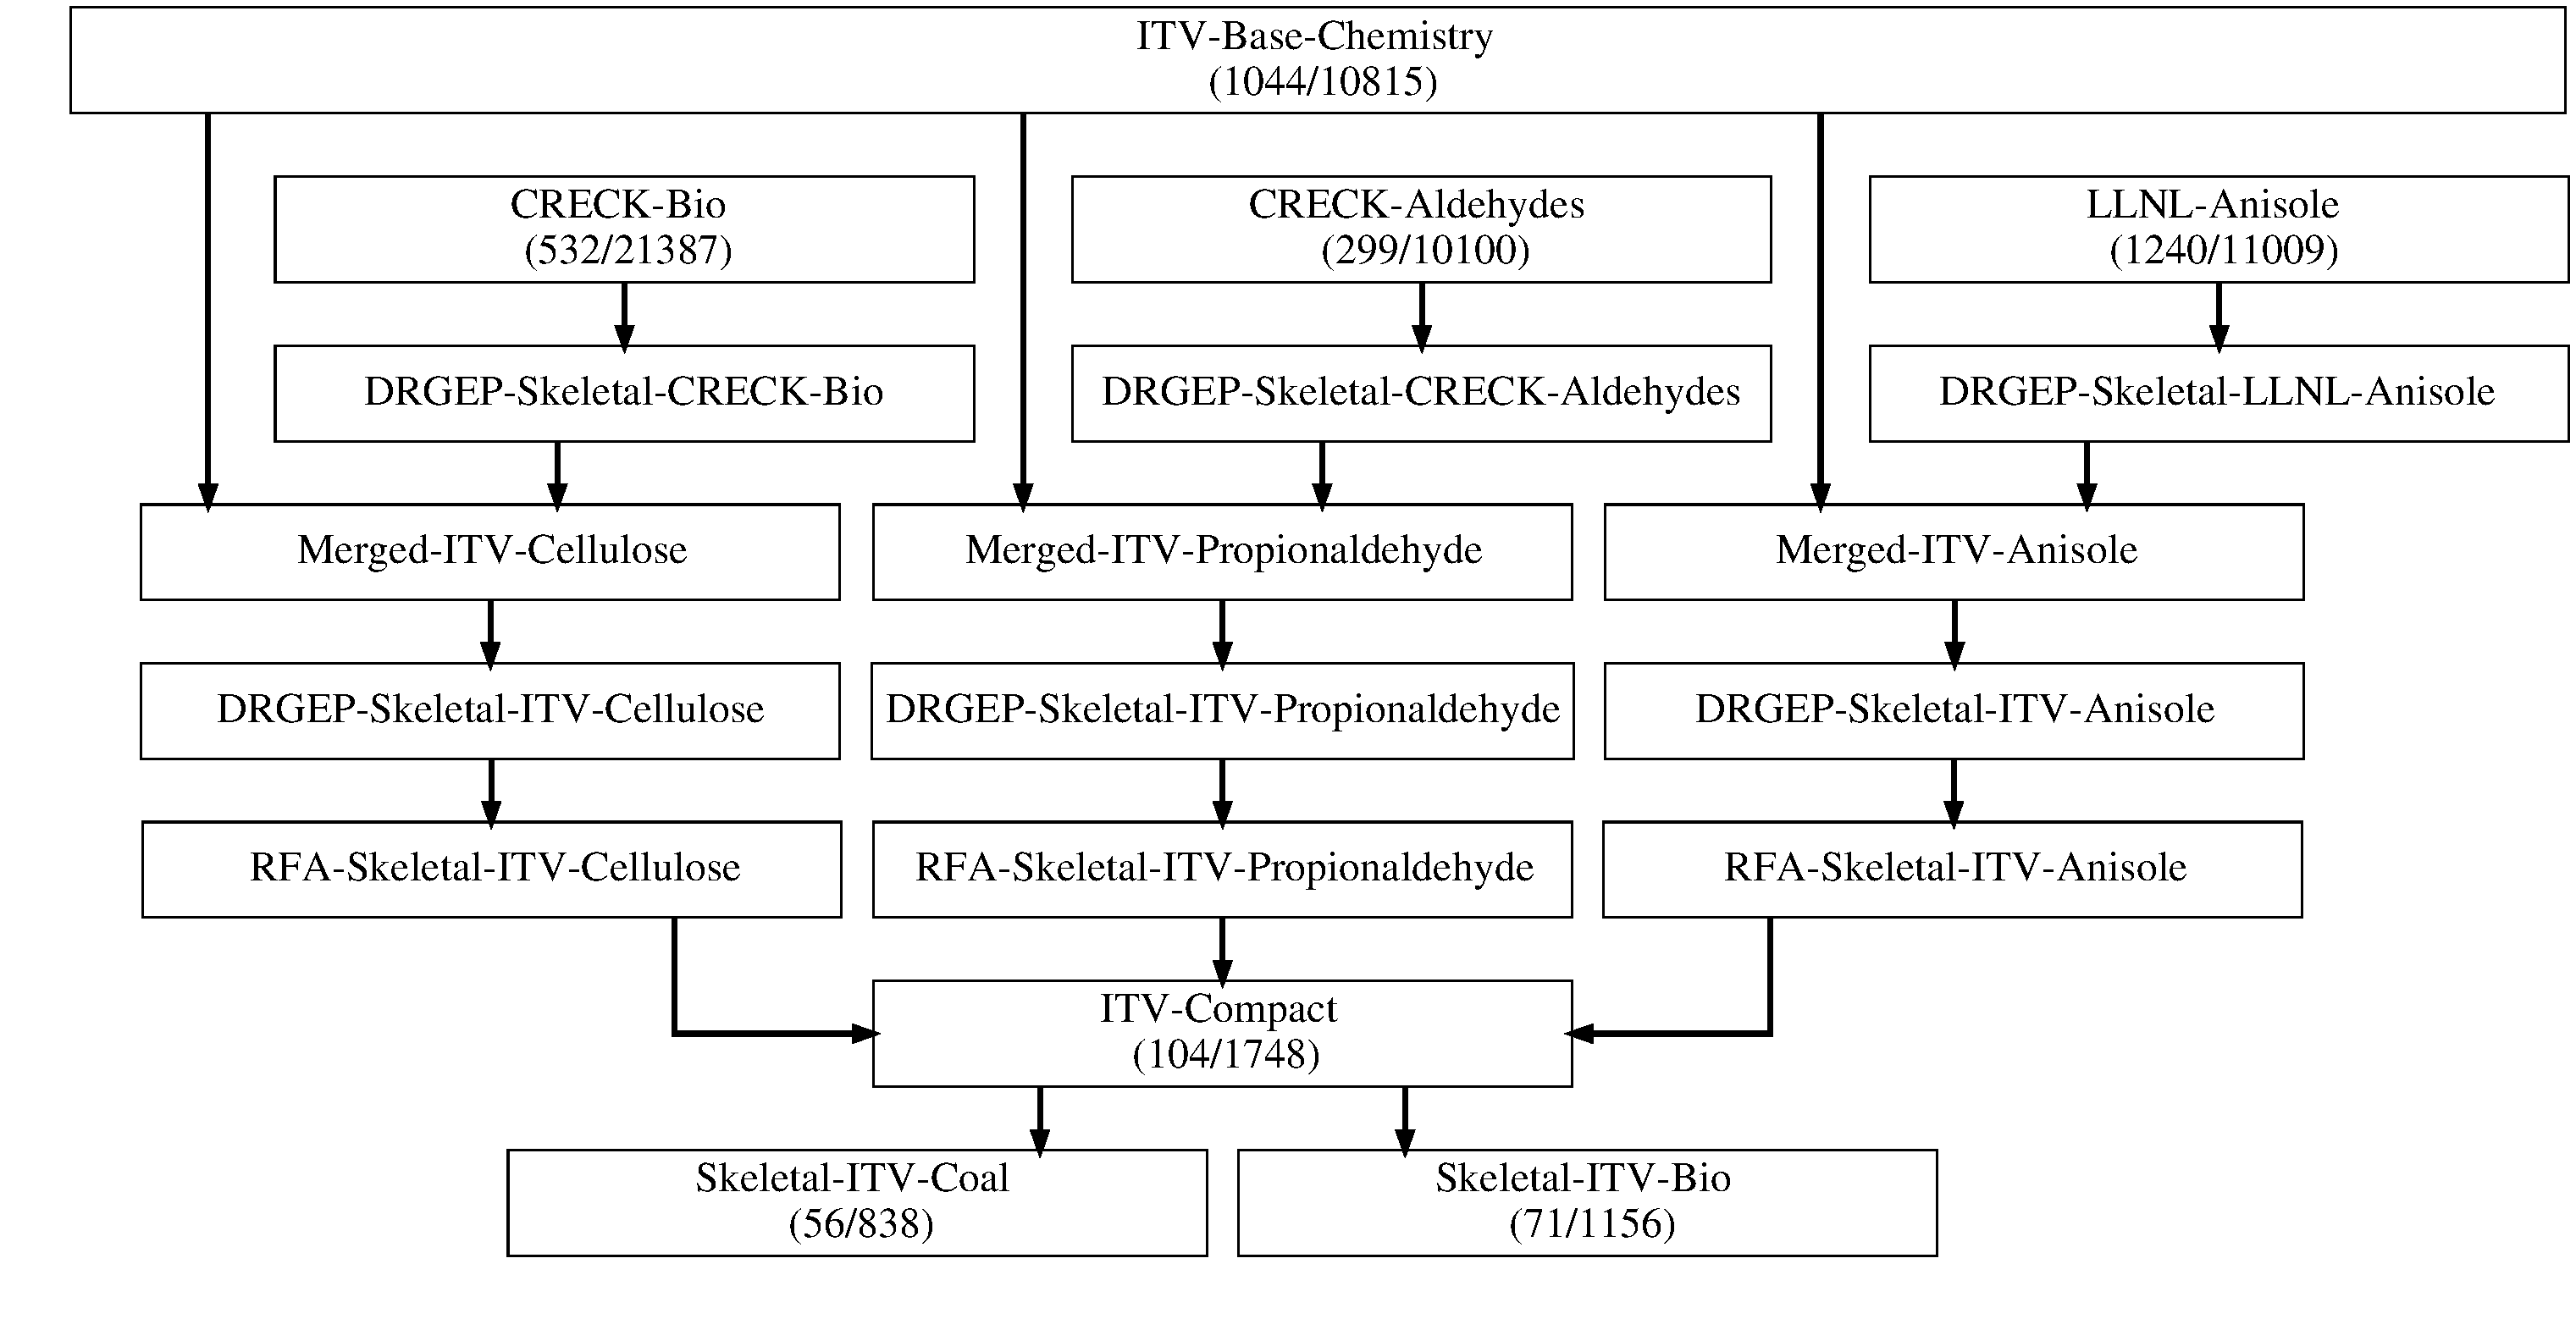
\includegraphics[width=1.0\textwidth]{\ThisPath Figures/B1b_FlowChartMechanismDevelopment.pdf}}
  \caption{Flow chart for developing the skeletal gas phase mechanisms for coal (Skeletal-ITV-Coal) and biomass (Skeletal-ITV-Bio) combustion. The initial mechanisms are the ITV-Base-Chemistry from Langer et al.~\cite{Langer2023}, the LLNL-Anisole~\cite{Wagnon2018}, the CRECK-Bio~\cite{Debiagi2016}, and the CRECK-Aldehydes model~\cite{Pelucchi2015}.}
  \label{fig:B1bKineticModelDevelopmentStructure}
\end{figure}
\\
Further DRGEP reduction steps of these mechanisms using the same validation cases lead to skeletal chemical kinetic mechanisms. A reaction flux analysis allows a flexible and targeted extraction of major formation and consumption pathways of the species of interest from the mechanism. The theory of both methods is described later in this section. The extraction with the reaction flux analysis was performed based on the respective validation cases to consider the range of validity and application. The extracted models for anisole oxidation, cellulose pyrolysis, and propionaldehyde chemistry are merged into an intermediate model to obtain a model that can describe all these features.
\\
A compact chemical kinetic model (ITV-Compact) is obtained to capture the prediction for all validation cases for coal and biomass combustion. This model can be used for further mechanism reductions for coal and biomass combustion. The species vanillin and the decomposition reaction for vanillin were added to this compact mechanism from the ITV-Base-Chemistry model~\cite{Langer2023} since it is a major volatile for coal and biomass combustion. Furthermore, isomers of 5-methyl-1,3-cyclopentadiene and the methylcyclopentadienyl radical were lumped based on the approach from Pepiot-Desjardins and Pitsch~\cite{PepiotDesjardins2008b}. The ITV-Compact mechanism contains several volatile species released from the CRECK-S model, which can be used to model coal and biomass combustion and as a basis for further reduction steps.
\\
The final reduction step contains a DRGEP step and an additional reduction step using the reaction flux analysis to obtain skeletal chemical kinetic models for coal and biomass combustion. The applicability of both models can be emphasized by the fact that the Skeletal-ITV-Coal and the Skeletal-ITV-Bio mechanisms contain several volatile species released from the CRECK-S model.

 
\subsubsection{Detailed chemical kinetic models}
Skeletal kinetic models aim to reproduce combustion characteristics exhibited by detailed models within a specified set of conditions. The latter should be selected to encompass the validity range of the detailed model. From this perspective, having access to a detailed model with strong predictive capabilities across a broad spectrum of experimental conditions constitutes a crucial step in developing a reliable skeletal kinetic model.
\\
In this project, a compact model describing the gas phase kinetics of coal and biomass combustion has been developed by integrating the relevant chemistry of missing volatile species in the extensively validated detailed model from Langer et al.~\cite{Langer2023}. The model from Langer et al.~\cite{Langer2023} is developed to describe the formation of PAH, suitable to describe the soot formation behaviour from biomass combustion. According to the CRECK-S devolatization model described in Cha.~\ref{sec:\Project_A8}, coal and biomass particles release a complex mixture of volatile species to the gas phase. One of the dominant volatile species released during coal and lignin combustion is anisole. During cellulose combustion, levoglucosan is the dominant volatile species released, while propionaldehyde is the most dominant species released at particle temperatures where biomass ignites is observed. However, these species are not included in the detailed model from Langer et al.~\cite{Langer2023}. To integrate these missing species chemistry in the model from Langer et al.~\cite{Langer2023}, extensively validated detailed chemical kinetic models describing the respective chemistry of interest over a broad range of conditions are used. The missing anisole chemistry has been adopted from the model of Wagnon et al.~\cite{Wagnon2018}, cellulose volatile species from Debiagi et al.~\cite{Debiagi2016}, and the propionaldehyde chemistry from Pelucchi et al.~\cite{Pelucchi2015}.
\\
The integration of the chemistry describing the gas-phase kinetics of these volatile species into the model from Langer et al.~\cite{Langer2023} has been achieved using a systematic approach. In order to extrapolate only the relevant chemistry for the species, the DRGEP method has been applied to these detailed models. The obtained reduced chemical kinetic models are merged into the detailed model from Langer et al.~\cite{Langer2023} based on InChIs and SMILES for each species, while only the species and reactions, as well as the species thermodynamic and transport data, were extracted and added to the chemical kinetic model from Langer et al.~\cite{Langer2023}, which are not included.
\\
The validation database presented in Ref.~\cite{Langer2023} is expanded in this work by integrating additional speciation data representative of anisole oxidation~\cite{Chen2022}, levoglucosan pyrolisis~\cite{Norinaga2013}, and shock tube ignition-delay time measurements of anisole and propionaldehyde~\cite{Pelucchi2015, AkihKumgehBergthorson2011}. The latter has been selected as anisole and propionaldehyde, respectively, the dominant volatile species at the particle ignition during coal and biomass combustion based on model simulations with the solid particle models.
% Here add oxyfuel validation (!highlight oxyfuel compability!...)

 

\subsubsection{Skeletal chemical kinetic model}
The skeletal kinetic models for coal and biomass combustion will be developed and employed to simulate the gas-phase kinetics of the primary volatile species released during single-particle combustion of coal and biomass under high-temperature and atmospheric pressure conditions. The reduction stage aims to develop chemical kinetic models with a limited number of species while accurately describing the evolution of volatile species under the specific conditions of interest.
\\
However, there is often an opposite trend between the effectiveness of a given kinetic model reduction technique and its computational demand. Based on this, most reduction strategies often consist of faster approaches for reducing detailed chemical kinetic models, where only a species priority list is generated, and numerically more expensive techniques on already reduced models.
\\
Reaction flux-based reduction techniques, such as the DRG~\cite{Lu2005, Lu2020} or DRGEP~\cite{PepiotDesjardins2008a} methods, have the advantage of being very fast in determining a species ranking. These graph-based methods can remove unimportant species from the chemical kinetic model and retain almost all their accuracy. However, increasing the threshold for the reduction leads to an accuracy loss, and the method progressively loses effectiveness. In contrast, a numerically more expensive sensitivity analysis is often applied to reduce skeletal chemical kinetic models. A sensitivity analysis calculates the error on a specific defined target following the removal of each analysed species and ranks them accordingly.
\\
Due to the underlying detailed chemical kinetic models for developing the skeletal models, graph-based reduction techniques are employed to achieve a strongly reduced number of species. Graph-based methodologies allow to schematise the reaction network as a mathematical object, a directed weighted graph which is defined as
\begin{align}
G = \{e,v,w\},
\end{align}
where vertex $v$ represents the species, the edges $e$ connecting two vertexes are the reactions, and the weight $w$ defines the strength of the links connecting two species. The definition of the weights varies according to the adopted methodology.


\subsubsection{Directed relation graph with error propagation method}
The directed relation graph with error propagation method~\cite{PepiotDesjardins2008a} is a reliable tool for systematically reducing mechanisms to a skeletal version of itself. The strength of interaction between two directly related species $A$ and $B$ is given with the direct interaction coefficient
\begin{align}
r_{AB} \equiv \frac{|\sum_{j=1}^{N_R} \nu_{j,A}\omega_j\delta_{B}^{j}|}{max(P_A, C_A)},
\end{align}
where the production and consumption rates of target species $A$ are given with
\begin{align}
\label{eq:B1bProductionRate}
P_A = \sum_{j=1}^{N_R} max(0, \nu_{j,A}\omega_j),
\end{align}
\begin{align}
\label{eq:B1bConsumptionRate}
C_A = \sum_{j=1}^{N_R} max(0, -\nu_{j,A}\omega_j).
\end{align}
$N_\mathrm{R}$ is the number of reactions in the kinetic model, $\nu_\mathrm{j}$ is the stoichiometric coefficient, and $\omega_\mathrm{j}$ is the net reaction rate of reaction $j$. $\delta_{B}^{j}$ is unity if the $j$-th reaction involves species $B$ and equals zero otherwise. After calculating the interaction coefficients for all species pairs in the reaction network, a graph search is performed to find all paths from the target species. A path-dependent interaction coefficient on a certain path $p$ that links two species $A$ and $B$, which are not necessarily directly related, represents the error propagation and is defined through a damping procedure as
\begin{align}
r_{AB,p} = \prod_{i=1}^{n-1} r_{S_iS_{i+1}},
\end{align}
where $n$ is the number of species between target species $A$ and species $B$ in pathway $p$ ($S_\mathrm{1}$ = $A$, and $S_\mathrm{n}$ = $B$). The coefficient $R$ represents the introduced error if species $B$ is removed on the prediction of target species $A$ and is defined as the maximum of all path-dependent interaction coefficients between the target species $A$ and each species of interest $B$ of target simulations $T_\mathrm{sim}$:
\begin{align}
R_{AB} \equiv \mathop{max}_{T_{sim}} (\mathop{max}_{\text{all paths } p} (r_{AB,p})).
\end{align}
This target-oriented technique returns a set of species that can be removed from the detailed mechanism with minimal impact on the target species for the range of validity and applicability. The conditions defining the range of validity are both examined counterflow flames from Chen et al.~\cite{Chen2022} measured in the burner from Cha.~\ref{\Project_B1} for the anisole oxidation chemistry, the secondary pyrolysis of cellulose volatiles species from Norinaga et al.~\cite{Norinaga2013}, and the ignition delay time measurements for propionaldehyde from Pelucchi et al.~\cite{Pelucchi2015} and Akih-Kumgeh and Bergthorson~\cite{AkihKumgehBergthorson2011}. The ignition delay time for anisole was validated with anisole/air mixtures at atmospheric pressure. The target species for the DRGEP reduction step were the respective volatile species and additional small \ce{C1} and \ce{C2} hydrocarbons.


\subsubsection{Reaction flux analysis}
Reaction flux analysis generally visualizes the main pathways consuming or producing a certain species. In this mechanism development, the reaction flux analysis tool is employed further to decrease the size of the chemical kinetic model. Unlike the DRGEP method, where the coefficient assigned to a certain species is maximum over all the validation cases, we will ensure that the neglected portion of the reaction network will be the same over the validation cases.
\\
For a species of interest, a directed graph is created based on the chemical kinetic model to highlight production or consumption pathways, where the vertices are species, and the edges refer to the integrated net reaction flux linking two species. The reaction flux for the production and consumption of a target species $A$ is defined as
\begin{align}
r_{AB} \equiv \frac{|\sum_{j=1}^{N_R} max(0; P_{A,j})\delta_{B}^{j}|}{\sum_{j=1}^{N_R} max(0; P_{A,j})},
\end{align}
\begin{align}
r_{AB} \equiv \frac{|\sum_{j=1}^{N_R} max(0; C_{A,j})\delta_{B}^{j}|}{\sum_{j=1}^{N_R} max(0; C_{A,j})}.
\end{align}
The directed graph is built based on the depth-first-search approach to ensure that every traversed pathway connects target species $A$ with any other species. The direction of the directed graph coincides with the direction of the net reaction rate for consumption or production pathways, respectively. Since all pathways contribute directly or indirectly to the consumption or formation of a target species, a tolerance is defined to consider only the most relevant pathways in the directed graph for the target species $A$. The error propagation approach in the reaction flux analysis is similar to the DRGEP method.
\\
A target species' dominant consumption or production pathways can be extracted from the directed graph based on a simulation that defines the range of applications. However, the remaining fluxes can be neglected from the model without changing the consumption or formation of the target species in the range of validity and applicability. The applied validation simulations defining the range of validity of the skeletal models are the same as those used for the DRGEP method reduction steps. The target species for the reaction flux analysis are the fuel and main pollutants for the ignition delay time extraction, while for the anisole and cellulose chemistry, a more detailed extraction process is applied, considering several small intermediate species as targets with different tolerances.


\subsection{Development of a \ce{NOx} chemical kinetic submodel}
To describe the formation of \ce{NO_x} from nitrogen-containing volatile species released from the CRECK-S model, a chemical kinetic gas-phase model for \ce{NO_x} formation is newly developed. This newly developed chemical kinetic model uses an ITV-\ce{NO_x} model, a reduced version of the well-documented Glarborg et al. model~\cite{Glarborg2018}, crafted through ab-initio and experimental studies, as base chemistry. Based on a quantitative assessment of ammonia and ammonia/hydrogen combustion of different chemical kinetic models, Girhe et al.~\cite{Girhe2024} reported satisfactory results under most of the examined experimental conditions for the KAUST ammonia model~\cite{Zhang2021}. Based on this study, the ITV integrates the ammonia chemistry from the KAUST model to the reduced Glaborg model to improve the predictions of the ammonia chemistry. The required pyridine chemistry to model tar-N is adopted from the CRECK-\ce{NO_x} model~\cite{Shamooni2021} and integrated into the base-chemistry model from the ITV.
\\
However, this merged ITV-\ce{NO_x} model over-predicts the \ce{NO} formation over a broad range of experimental conditions. Comparing the \ce{NO} formation pathways from the ITV-\ce{NO} model and the CRECK-\ce{NO_x} model~\cite{Shamooni2021}, which is able to capture the \ce{NO} formation accurately, reveals an over-predicted \ce{NCO}-chemistry in the ITV-\ce{NO_x} model. The dominant \ce{NO} formation reactions via the \ce{NCO} radical differ in both kinetic models, while the most dominant \ce{NCO} consumption reaction in the ITV-\ce{NO_x} model is
\begin{align}
\ce{NCO}+\ce{O} \Leftrightarrow \ce{NO}+\ce{CO}.
\end{align}
To slow down this \ce{NO} formation pathway, the tuned reaction rate from the CRECK-\ce{NO_x} model~\cite{Shamooni2021} is adopted to the ITV-\ce{NO_x} model. With this reaction rate modification, the \ce{NCO} pathway is slowed down and the \ce{NH}-chemistry becomes more important for the \ce{NO} formation, resulting in an accurately predicted NO formation. However, this modification results in an over-predicted \ce{N2O}-chemistry. A slightly reduced frequency parameter for the most dominant \ce{N2O} formation reaction in the ITV-\ce{NO_x} model
\begin{align}
\ce{NCO}+\ce{NO} \Leftrightarrow \ce{N2O}+\ce{CO},
\end{align}
slows down this \ce{N2O} formation pathway and results in an accurate \ce{N2O} prediction.
\\
Next to the rate modifications, the nitrogen chemistry in the ITV model is extracted using the reaction flux analysis to obtain a more compact model size. The target species for the extraction are the volatile species released from the solid particle models. Using a very tiny tolerance for the flux analysis and considering the validation cases from Alzueta et al.~\cite{Alzueta2002} and Wu et al.~\cite{Wu2019, Wu2022}, an extracted kinetic model is obtained, which covers a broad spectrum of fuel-air ratios, temperatures, and initial conditions. The extracted model is a generally applicable modular chemical kinetic model for \ce{NO_x} formation containing 36 species and 595 reactions.
% R1 not Eq????


%%%%%%%%%%%%%%%%%%%%
% Mittwoch:
% - figures creten and adden to validation chapter (erst meine danach auch L.Cai (reproducen with FM)
% - Introduction 1.1 and 1.3
% Donnerstag:
% - schreiben Validation chapter
% Freitag:
% 1.2.1 Liming Cai ... & abstract
%%%%%%%%%%%%%%%%%%%%

\section{Validation of the kinetic models}
 % auch oxyfuel conditions 3 plots ...
 
\subsection{Skeletal kinetic model for coal combustion}
 
\subsubsection{ITV-2019}
Liming Cai model
 
\subsubsection{ITV-2023}
new model

\subsection{Skeletal kinetic model for biomass combustion}
 
\subsection{Validation of \ce{NOx} chemical kinetic submodel}






%%%% DON'T CHANGE ANYTHING FROM HERE UNTIL NEXT MARKER!
\Acknowledgement

%\ThisPath 
\renewcommand{\bibname}{References}
\printbibliography[heading=subbibliography]

\end{refsection}
%%%% DONT CHANGE ANYTHING UNTIL HERE!
